% Performance matrix for QEDRank run 2026-10-11-466b32a
% Generated by paper/make-tex.cjs from the run's item records on 2026-10-11.
% Rebuild after a re-grade:  node paper/make-tex.cjs runs/<run-id> paper/performance-matrix.tex
%
% Each table and figure below is self-contained: copy the environments you need into the paper and
% add these packages and colours to its preamble.
\documentclass[11pt]{article}
\usepackage[a4paper,margin=2.2cm]{geometry}
\usepackage[T1]{fontenc}
\usepackage{lmodern}
\usepackage{booktabs}
\usepackage{tabularx}
\usepackage{array}
\usepackage{threeparttable}
\usepackage[font=small,labelfont=bf]{caption}
\usepackage{xcolor}
\usepackage{pgfplots}
\pgfplotsset{compat=1.18}
\definecolor{qrTimeout}{RGB}{110,110,110}
\definecolor{qrRate}{RGB}{175,175,175}
\definecolor{qrAbst}{RGB}{86,180,233}
\definecolor{qrEnv}{RGB}{230,159,0}
\definecolor{qrImp}{RGB}{240,228,66}
\definecolor{qrScreen}{RGB}{153,153,51}
\definecolor{qrErr}{RGB}{213,94,0}
\definecolor{qrStmt}{RGB}{204,121,167}
\definecolor{qrSorry}{RGB}{0,114,178}
\definecolor{qrAx}{RGB}{100,50,120}
\definecolor{qrOk}{RGB}{0,158,115}
\newcommand{\swatch}[1]{\textcolor{#1}{\rule{0.75em}{0.75em}}}

\begin{document}

\section*{Pilot evaluation: performance matrix}
Run \texttt{2026-10-11-466b32a}, 111 ProofBench problems, task \emph{prove the given statement}, 2 models.

% ---------------------------------------------------------------- Table: setup
\begin{table}[!htbp]
\centering
\caption{Evaluation setup of run \texttt{2026-10-11-466b32a}.}
\label{tab:setup}
\small
\begin{tabularx}{\linewidth}{@{}>{\raggedright\arraybackslash}p{2.4cm}>{\raggedright\arraybackslash}X@{}}
\toprule
Corpus & \texttt{proofbench-statements} at commit \texttt{466b32a} (2026-10-08): 111 problems with a main-theorem target; claim status 80 established, 30 open, 1 uncertain. The 28 disproof variants were not evaluated. \\
Task & Prove the given statement: the model receives the challenge file, whose main theorem ends in a single \texttt{sorry}, and must return the completed file with the statement and all definitions unchanged. \\
Protocol & One request per problem (pass@1), no repair rounds, no tools or retrieval; prompt template \texttt{qedrank-prove-v1}. \\
Models & \textbf{Kimi K3}: \texttt{kimi-k3} via \texttt{api.moonshot.ai}; 2.8\,T parameters, 104\,B active (mixture of experts); released 2026-07-16; temperature set by the provider.\newline \textbf{Qwen3-30B-A3B}: \texttt{qwen3-30b-a3b-instruct-2507} via \texttt{chat-ai.academiccloud.de}; 30.5\,B parameters, 3.3\,B active (mixture of experts); released 2025-07-30; temperature 0. \\
Budgets & 16{,}384 output tokens and 300\,s per request. \\
Grader & Lean v4.34.1, Mathlib \texttt{d13f23b}; 400{,}000 heartbeats, 600\,s and 8\,GB per compilation. A solution counts as verified when it compiles, contains no \texttt{sorry}, keeps the main theorem and every challenge definition unchanged as compiled declarations, uses only \texttt{propext}, \texttt{Classical.choice} and \texttt{Quot.sound}, and replays through the kernel.\textsuperscript{a} \\
Harness & QEDRank commit \texttt{65375e7f63}; total wall-clock time 4.3\,h. \\
Statistics & Exact two-sided 95\,\% Clopper--Pearson intervals. Each problem contributes one item, so clustering by paper does not change the intervals. \\
\bottomrule
\end{tabularx}
\par\smallskip\parbox{\linewidth}{\footnotesize \textsuperscript{a}\,This run was graded in the QEDRank default Lean project (\texttt{lean}). The benchmark pins Lean v4.33.1, Mathlib v4.33.1, the Matroid library at \texttt{fa6c155} and the option \texttt{maxSynthPendingDepth = 3}, and its problem library \texttt{ProofBench.Mathlib\_Problems} was not on the grader's search path.}
\end{table}

% ---------------------------------------------------------------- Table: outcome breakdown
\begin{table}[!htbp]
\centering
\caption{Outcome of every request, by model (111 problems each). Categories are mutually exclusive; each item is assigned to the first step at which it stopped.}
\label{tab:outcomes}
\small
\begin{tabular}{@{}lrr@{}}
\toprule
Outcome & Kimi K3 & Qwen3-30B-A3B \\
\midrule
\addlinespace[2pt]\multicolumn{3}{@{}l}{\textit{Provider}} \\
\quad\swatch{qrTimeout}\,Request timed out (300 s) & 37 (33.3\,\%) & 0 (0.0\,\%) \\
\quad\swatch{qrRate}\,Rate limited (HTTP 429) & 57 (51.4\,\%) & 0 (0.0\,\%) \\
\addlinespace[2pt]\multicolumn{3}{@{}l}{\textit{Grader configuration (not attributable to the model)}} \\
\quad\swatch{qrEnv}\,Problem library missing from grader & 2 (1.8\,\%) & 48 (43.2\,\%) \\
\quad\swatch{qrImp}\,Challenge import rejected by policy & 0 (0.0\,\%) & 11 (9.9\,\%) \\
\addlinespace[2pt]\multicolumn{3}{@{}l}{\textit{Model}} \\
\quad\swatch{qrAbst}\,Abstained (no Lean file returned) & 15 (13.5\,\%) & 2 (1.8\,\%) \\
\quad\swatch{qrErr}\,Lean compile error & 0 (0.0\,\%) & 46 (41.4\,\%) \,{\footnotesize(30 cut off)} \\
\quad\swatch{qrStmt}\,Compiled; target statement changed or absent & 0 (0.0\,\%) & 1 (0.9\,\%) \\
\quad\swatch{qrSorry}\,Compiled; proof contains \texttt{sorry} & 0 (0.0\,\%) & 3 (2.7\,\%) \\
\quad\swatch{qrOk}\,Verified & 0 (0.0\,\%) & 0 (0.0\,\%) \\
\midrule
Total & 111 & 111 \\
\bottomrule
\end{tabular}
\par\smallskip\parbox{0.92\linewidth}{\footnotesize \textit{Cut off}: the answer reached the 16{,}384-token output limit before it ended. \textit{Problem library missing}: the challenge imports \texttt{ProofBench.Mathlib\_Problems}, which the grader's Lean project did not contain. \textit{Challenge import rejected}: the import policy rejected an import that the challenge file itself contains (the Matroid library, \texttt{Archive}, or another problem's module); the model added no import.}
\end{table}

% ---------------------------------------------------------------- Figure: outcome composition
\begin{figure}[!htbp]
\centering
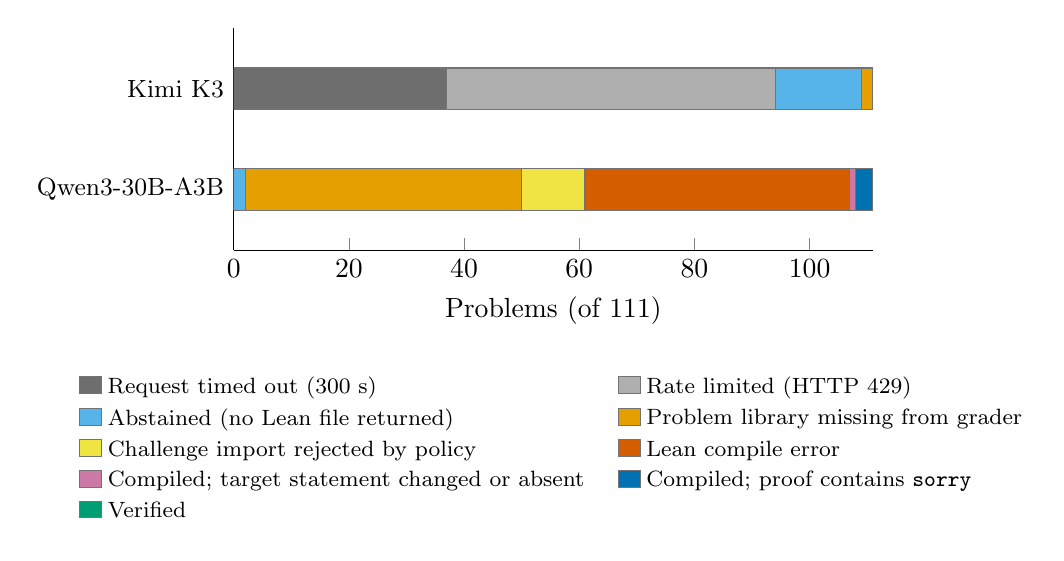
\begin{tikzpicture}
\begin{axis}[
  xbar stacked, bar width=15pt, width=0.8\linewidth, height=4.4cm,
  xmin=0, xmax=111, xlabel={Problems (of 111)},
  ytick={0,1}, yticklabels={Qwen3-30B-A3B,Kimi K3},
  ymin=-0.6, ymax=1.6, y tick label style={font=\small},
  legend style={at={(0.5,-0.52)}, anchor=north, legend columns=2, draw=none, font=\footnotesize,
    /tikz/every even column/.append style={column sep=10pt}},
  legend cell align=left, axis x line*=bottom, axis y line*=left,
]
\addplot[fill=qrTimeout, draw=black!55] coordinates {(0,0) (37,1)};
\addplot[fill=qrRate, draw=black!55] coordinates {(0,0) (57,1)};
\addplot[fill=qrAbst, draw=black!55] coordinates {(2,0) (15,1)};
\addplot[fill=qrEnv, draw=black!55] coordinates {(48,0) (2,1)};
\addplot[fill=qrImp, draw=black!55] coordinates {(11,0) (0,1)};
\addplot[fill=qrErr, draw=black!55] coordinates {(46,0) (0,1)};
\addplot[fill=qrStmt, draw=black!55] coordinates {(1,0) (0,1)};
\addplot[fill=qrSorry, draw=black!55] coordinates {(3,0) (0,1)};
\addplot[fill=qrOk, draw=black!55] coordinates {(0,0) (0,1)};
\legend{{Request timed out (300 s)},{Rate limited (HTTP 429)},{Abstained (no Lean file returned)},{Problem library missing from grader},{Challenge import rejected by policy},{Lean compile error},{Compiled; target statement changed or absent},{Compiled; proof contains \texttt{sorry}},{Verified}}
\end{axis}
\end{tikzpicture}
\caption{Where each request ended. Grey: provider failures; orange and yellow: answers the grader could not evaluate because of its configuration; the remaining colours are outcomes attributable to the model (Table~\ref{tab:outcomes}).}
\label{fig:outcomes}
\end{figure}

% ---------------------------------------------------------------- Table: performance matrix
\begin{table}[!htbp]
\centering
\begin{threeparttable}
\caption{Performance matrix on the main theorems (task: prove the given statement, pass@1). Rates exclude provider failures and items the grader could not evaluate.}
\label{tab:matrix}
\small
\begin{tabular}{@{}lrr@{}}
\toprule
Measure & Kimi K3 & Qwen3-30B-A3B \\
\midrule
Problems run & 111 & 111 \\
Requests timed out & 37 & 0 \\
Requests refused (HTTP 429) & 57 & 0 \\
Answered & 17 & 111 \\
Abstained\tnote{b} & 15/17 (88.2\,\%) & 2/111 (1.8\,\%) \\
Answer cut off at token limit & 0/17 (0.0\,\%) & 66/111 (59.5\,\%) \\
Not gradable (grader configuration)\tnote{a} & 2 & 59 \\
Graded proof attempts & 0 & 50 \\
\midrule
Compile rate\tnote{c} & --- & 4/50 (8.0\,\%) \\
\quad 95\,\% CI & --- & [2.2, 19.2] \\
Statement unchanged (of compiled) & --- & 3/4 (75.0\,\%) \\
No \texttt{sorry}, standard axioms (of compiled) & --- & 0/4 (0.0\,\%) \\
\textbf{Verified pass@1}\tnote{d} & \textbf{0/8 (0.0\,\%)} & \textbf{0/43 (0.0\,\%)} \\
\quad 95\,\% CI & [0.0, 36.9] & [0.0, 8.2] \\
\midrule
Compile rate, as graded\tnote{e} & 0/2 (0.0\,\%) & 4/109 (3.7\,\%) \\
Verified pass@1, as graded\tnote{e} & 0/8 (0.0\,\%) & 0/80 (0.0\,\%) \\
\midrule
Median latency per answer & 146.7\,s & 81.5\,s \\
Median output tokens per answer & 5{,}444 & 16{,}384 \\
\bottomrule
\end{tabular}
\begin{tablenotes}\footnotesize
\item[a] The grader could not evaluate the answer: the problem library was missing from its Lean project, or its import policy rejected an import of the challenge file itself (Table~\ref{tab:outcomes}). These items are excluded from every rate.
\item[b] Answered without a Lean file. A Lean file that leaves the \texttt{sorry} in place is counted as compiled with \texttt{sorry}, not as an abstention.
\item[c] Graded attempts whose file compiled without errors. A compiling file is not a success.
\item[d] Compiles, contains no \texttt{sorry}, keeps the main theorem and all challenge definitions unchanged as compiled declarations, depends only on the standard axioms, and replays through the kernel. Denominator: problems whose claim is established, excluding provider failures and items that could not be graded; abstentions count as failures.
\item[e] The grader's own figures, before items it could not evaluate are removed; reported for comparison only.
\item[] Kimi K3: the 17 answered problems are those that finished within the time limit before the rate limit set in, so its abstention rate is not representative. No comparison between the models is made.
\end{tablenotes}
\end{threeparttable}
\end{table}

% ---------------------------------------------------------------- Figure: funnel
\begin{figure}[!htbp]
\centering
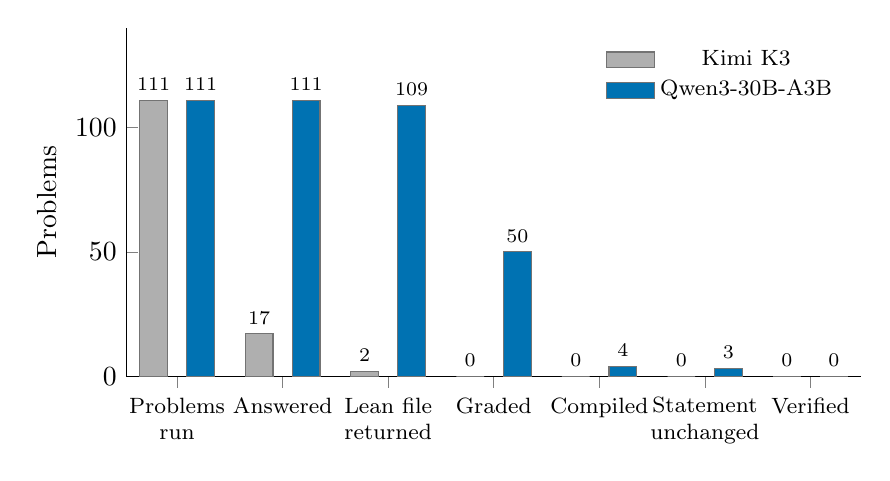
\begin{tikzpicture}
\begin{axis}[
  ybar=7pt, bar width=10pt, width=0.9\linewidth, height=6cm, area legend,
  ymin=0, ymax=140, ylabel={Problems},
  xtick={1,...,7}, xticklabels={{Problems\\run},{Answered},{Lean file\\returned},{Graded},{Compiled},{Statement\\unchanged},{Verified}},
  xticklabel style={align=center, font=\footnotesize}, enlarge x limits=0.08,
  nodes near coords, every node near coord/.append style={font=\scriptsize},
  legend style={at={(0.98,0.97)}, anchor=north east, draw=none, font=\footnotesize},
  axis x line*=bottom, axis y line*=left,
]
\addplot[fill=qrRate, draw=black!55] coordinates {(1,111) (2,17) (3,2) (4,0) (5,0) (6,0) (7,0)};
\addplot[fill=qrSorry, draw=black!55] coordinates {(1,111) (2,111) (3,109) (4,50) (5,4) (6,3) (7,0)};
\legend{Kimi K3,Qwen3-30B-A3B}
\end{axis}
\end{tikzpicture}
\caption{Attrition from request to verified proof. \emph{Graded} counts the returned files that the grader could evaluate; the drop from \emph{Lean file returned} to \emph{Graded} is caused by the grader configuration, not by the model.}
\label{fig:funnel}
\end{figure}

% ---------------------------------------------------------------- Figure: output length
\begin{figure}[!htbp]
\centering
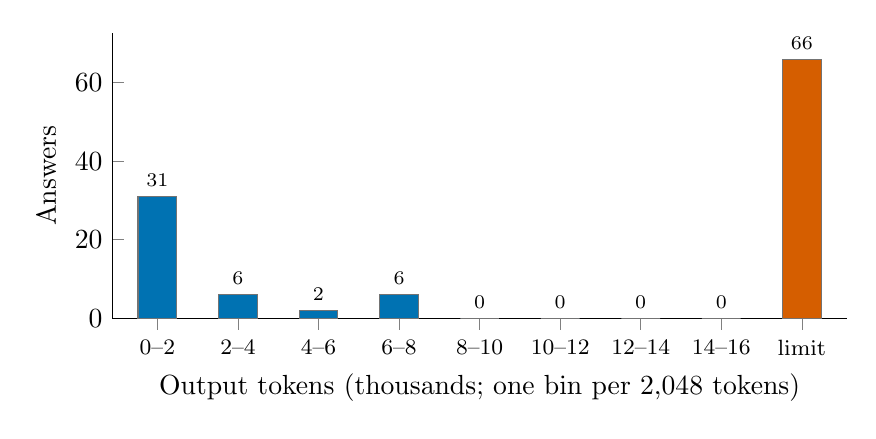
\begin{tikzpicture}
\begin{axis}[
  ybar, bar width=14pt, width=0.9\linewidth, height=5.2cm,
  ymin=0, ylabel={Answers}, xlabel={Output tokens (thousands; one bin per 2{,}048 tokens)},
  xtick={1,...,9}, xticklabels={0--2,2--4,4--6,6--8,8--10,10--12,12--14,14--16,limit}, xticklabel style={font=\footnotesize},
  nodes near coords, every node near coord/.append style={font=\scriptsize},
  enlarge x limits=0.07, axis x line*=bottom, axis y line*=left,
]
\addplot[fill=qrSorry, draw=black!55, bar shift=0pt] coordinates {(1,31) (2,6) (3,2) (4,6) (5,0) (6,0) (7,0) (8,0)};
\addplot[fill=qrErr, draw=black!55, bar shift=0pt] coordinates {(9,66)};
\end{axis}
\end{tikzpicture}
\caption{Length of the 111 answers of Qwen3-30B-A3B. 66 answers (59\,\%, right) reached the 16{,}384-token limit and were cut off before they ended.}
\label{fig:length}
\end{figure}

% ---------------------------------------------------------------- Figure: compile-error taxonomy
\begin{figure}[!htbp]
\centering
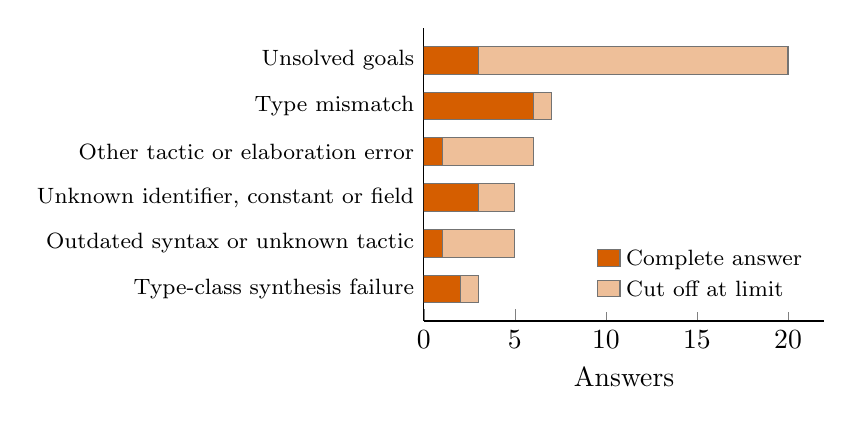
\begin{tikzpicture}
\begin{axis}[
  xbar stacked, bar width=10pt, width=0.55\linewidth, height=5.3cm,
  xmin=0, xlabel={Answers}, ytick={0,1,2,3,4,5},
  yticklabels={{Type-class synthesis failure},{Outdated syntax or unknown tactic},{Unknown identifier, constant or field},{Other tactic or elaboration error},{Type mismatch},{Unsolved goals}}, y tick label style={font=\footnotesize},
  ymin=-0.7, ymax=5.7,
  legend style={at={(0.98,0.03)}, anchor=south east, draw=none, fill=white, font=\footnotesize}, legend cell align=left,
  axis x line*=bottom, axis y line*=left,
]
\addplot[fill=qrErr, draw=black!55] coordinates {(2,0) (1,1) (3,2) (1,3) (6,4) (3,5)};
\addplot[fill=qrErr!40, draw=black!55] coordinates {(1,0) (4,1) (2,2) (5,3) (1,4) (17,5)};
\legend{Complete answer, Cut off at limit}
\end{axis}
\end{tikzpicture}
\caption{First Lean error of the 46 graded attempts of Qwen3-30B-A3B that failed to compile. Most \emph{unsolved goals} come from answers cut off at the token limit, where the proof stops mid-tactic.}
\label{fig:errors}
\end{figure}

% ---------------------------------------------------------------- Table: by difficulty
\begin{table}[!htbp]
\centering
\caption{Results by the benchmark's difficulty label (Qwen3-30B-A3B; the other model has no graded attempts).}
\label{tab:difficulty}
\small
\begin{tabular}{@{}lrrrrrr@{}}
\toprule
Difficulty label & Problems & Established & Not gradable & Graded & Compiled & Verified \\
\midrule
Calibration & 12 & 12 & 1 & 11 & 0 & 0 \\
Undergraduate & 2 & 2 & 1 & 1 & 0 & 0 \\
Research & 62 & 62 & 32 & 28 & 1 & 0 \\
Research, settled Oct 2026 & 4 & 4 & 3 & 1 & 0 & 0 \\
Open & 30 & 0 & 22 & 8 & 3 & 0 \\
Unlabelled & 1 & 0 & 0 & 1 & 0 & 0 \\
\bottomrule
\end{tabular}
\par\smallskip\parbox{0.9\linewidth}{\footnotesize \textit{Calibration} merges the benchmark's calibration labels (elementary to upper-end, with or without a Lean reference proof). \textit{Research, settled Oct 2026}: open until October 2026 and settled by a Lean-checked result announced on 6 October 2026 that had not been independently verified when the run was made.}
\end{table}

% ---------------------------------------------------------------- Table: compiled answers
\begin{table}[!htbp]
\centering
\caption{Every graded answer that compiled, and why none was verified.}
\label{tab:compiled}
\small
\begin{tabular}{@{}lll>{\raggedright\arraybackslash}p{4.6cm}l@{}}
\toprule
Problem & Model & Claim & Axioms of the main theorem & Outcome \\
\midrule
P009 & Qwen3-30B-A3B & open & --- & main theorem absent \\
P042 & Qwen3-30B-A3B & open & \texttt{propext}, \texttt{sorryAx}, \texttt{Classical.choice}, \texttt{Quot.sound} & \texttt{sorry} left in proof \\
P045 & Qwen3-30B-A3B & established & \texttt{propext}, \texttt{sorryAx}, \texttt{Classical.choice}, \texttt{Quot.sound} & \texttt{sorry} left in proof \\
P077 & Qwen3-30B-A3B & open & \texttt{propext}, \texttt{sorryAx}, \texttt{Classical.choice}, \texttt{Quot.sound} & \texttt{sorry} left in proof \\
\bottomrule
\end{tabular}
\end{table}

\clearpage
% ---------------------------------------------------------------- Threats to validity (adapt to the paper)
\subsection*{Threats to validity}
\begin{itemize}\setlength\itemsep{2pt}
\item \textbf{Grader configuration.} Both files returned by Kimi K3 and 59 of the 109 files returned by Qwen3-30B-A3B could not be evaluated, because the grader ran outside the benchmark's pinned Lean project and its import policy rejected imports that belong to the challenge files. The rates in Table~\ref{tab:matrix} therefore rest on 0 graded attempts (Kimi K3) and 50 graded attempts (Qwen3-30B-A3B). The answers that were graded were compiled with Lean v4.34.1 instead of the pinned v4.33.1 and without the benchmark's Lean options.
\item \textbf{Provider failures.} 94 of 111 requests to Kimi K3 failed (37 timed out after 300\,s; 57 were refused with HTTP 429 because the account allows one concurrent request). Its results are not comparable with the other model's.
\item \textbf{Single attempt.} One request per problem at temperature 0 where the provider allows it, without repair rounds or tools; pass@$k$ and repair success are not measured.
\item \textbf{Output budget.} 59\,\% of the answers of Qwen3-30B-A3B reached the 16{,}384-token limit (Figure~\ref{fig:length}); a larger budget could change its compile rate.
\item \textbf{Contamination.} Neither provider states a training cutoff and the problems' publication dates are not recorded, so prior exposure cannot be assessed.
\end{itemize}

\end{document}
